\ofsubsection{Optional Rules}
%
\ofquote{"Listen up! Teamwork means staying out of my way.\\ It's a Squad B rule."}{Seifer}
%
\vfill
%

\includegraphics[width=\columnwidth]{./art/images/ff7.jpg}
%
\vfill
%
You may decide to change the existing rules or add new rules to customize the game to your preferences.
We strongly encourage you to explore such ideas to optimize the rules for group's playstyle.
However, be aware that the game's content is designed around the default rules and we cannot guarantee that everything will work well once you change them.
Nevertheless, this subsection gives you some examples of interesting rule changes and additions to consider.
%
\vfill
%
\accf{Survival:}
The default rules do not focus on realism and survival, which should generally come second to existing fantasy elements.
However, with some small additions you can make your world significantly more unforgiving.\ofrow
\ofbullet{The inventory capacity of characters is limited to a total of 10 items or equipment pieces.}
\ofbullet{Characters who have not eaten properly in one day suffer DeATR for all attributes except AGI.}
\ofbullet{At night or inside unlit areas, characters permanently suffer Blind.}
\ofbullet{Character who have less than half of their maximum HP have Disadvantage on all checks.}
%
\vfill
%
\accf{Surrender:}
In some cases the party might want to resolve combat more peacefully than simply beating the enemies until they are KO.
The following rule allows players to conclude battles in a more graceful way:
a combatant can use his action to intimidate a target within 1u to surrender the battle.
In this case, the target performs a check and if he fails, he lays down his arms and stops fighting. 
The check usually has DC~7, but is increased to DC~10 if the target's current HP is less than 10\% of his maximum HP.
However, the check always succeeds if either the target's current HP is more than half of his maximum HP or if he has at least as many allies as enemies within 3u.
%
\newpage
%
\ofquote{"I can't stop thinking about dark knights! They're cool, and by cool, I mean totally sweet!"}{Young Villager}
%
\vfill
%
\accf{Unrestricted Archetypes:}
With this rule, you may allow for more customization in the job system:
when players select an Archetype for their character, they may select an Archetype from any job instead of just the ones from their own jobs.
%
\vfill
%
\accf{Experience Points:}
You can use an experience point system to track character experience instead of the default milestone based scheme. 
In this system, each party member gains one experience point per Level of an enemy defeated in combat, for example every party member is awarded 10 points when a Level 10 enemy is defeated.
In addition, you can award the party experience points for other achievements such as completing certain tasks.
The table below shows how many total experience points a character needs to reach a certain Level, which you can modify as you see fit.
%
\ofgap
%
\oftable{p{0.35\columnwidth} l}
{\accf{Level} & \accf{Cumulative Experience Points}}
{
	1 & 0 \\
	2 & 20 \\
	3 & 50 \\
	4 & 100 \\
	5 & 175 \\
	6 & 300 \\
	7 & 450 \\ 
	8 & 600 \\
	9 & 800 \\
	10 & 1000\\
}
%
\vfill
%
\accf{Equipment Upgrades:}
This rule allows player characters to upgrade their weapons and armor to higher equipment classes.
Upgrading an equipment piece from Beginner to Advanced class costs 1000G and from Advanced to Expert costs 2000G worth of materials.
The GM may enforce additional restrictions on upgrades, such as requiring specific materials or expertise to complete them.
Alternatively, the party may seek out a smith with enough expertise to perform the upgrade.
%
\vfill
%
\accf{Cinematic Finishers:}
This rule allows you to put additional emphasis on heroic moments in combat.
Whenever a player character causes KO to an enemy with a Critical Hit, Limit Break, Summon or by using a Fortune Die, they can perform a special finishing move.
In this case, the player describes in detail how his character finishes off the enemy and if he wants he can also strike a pose or utter a cheesy one-liner afterwards.
All enemies on the battlefield then make a DC~8 check and everyone who fails becomes frightened and cannot target the player character on their next turn.
%
\clearpage
%
\ofquote{"Once Lady Yuna fixes her hair, we leave."\\}{Auron}
%
\vfill
%
\accf{Short Rests:}
When the players have to face many challenging combat encounters per day, they may struggle with sustaining themselves.
You can use the following rule to provide the party with an additional tool that dampens the stress of long days.
Characters can take a short rest for 30 minutes to regain half of their maximum HP and MP. 
A party can take up to 3 such rests per day, and any further short rests afterward have no effect.
%
\vfill
%
\accf{Unlimited Progression:}
Characters usually cannot increase in Levels past a total of 10, but you can remove this limitation to allow for further progression.
Accordingly, only the most powerful antagonists will be able to provide a challenge to such a high Level party.
We recommend to use this rule in conjunction with the Job Change rule to allow characters to progress past Level 10 by mastering different aspects of combat.
%
\vfill
%
\accf{Job Change:}
This rule allows character's to change their job, but only once during the adventure after reaching a Level up.
Instead of increasing the Level of his or her old job, your character starts at Level~1 in the new job.
When changing your character's job, he or she keeps all of the learned abilities, attribute improvements and equipment expertise from the old job.  
The only exception to this is the AGI attribute, where your character only gains the higher bonus between the two jobs.
However, your character can only have a total maximum of 10 Levels between both jobs.
Accordingly, the flexibility of changing jobs comes at the cost of not being able to become an expert in either one.
%
\vfill
%
\ofboxwithtitle{Example: Job Change}{
	After fighting through the Wind Shrine and reaching its top, Bartz and his party realize that the Wind Crystal has already been destroyed.
	Regardless, the GM awards the party with a Level Up and everyone in the party except Bartz advances from Level 2 to 3.
	Bartz picks up one of the crystal shards and suddenly feels a rush of energy, which imbues him with magical powers.
	Instead of leveling up, he changes his job into Black Mage, starting at Level 1.
	Nevertheless, he keeps his attributes and the ability to equip swords and armor from his old Warrior job.
	In addition, his attributes	are increased as noted in the job description for Level 1 Black Mages.
	The only exception is the AGI attribute, which he keeps from its old job since it is higher.
	Bartz also learns the spells "Fire", "Ice" and "Lightning" in addition to the "Rush" and "Beatdown" Techs that he already knows.
}
%
\newpage
%
\accf{Legendary Equipment:}
Apart from normal weapons and armor, there is a special class of equipment that may exist in your world called the Legendary Equipment.
These are extraordinarily powerful weapons and armor with great relevance to the game world and accordingly tremendous effort is required to find them.
Legendary Equipment pieces are always unique and can only be wielded by Level 10 characters.
Legendary Weapons provide 4d DMG, Legendary Armor provide DEF~+3 and RES~+3, but they are still subject to specific rules of their type.
Below is a list of all legendary equipment pieces.
%
\vfill
%
\oftable{p{0.2\columnwidth} p{0.14\columnwidth} p{0.55\columnwidth}}
{\accf{Weapon} & \accf{Type} & \accf{Effect}}
{
	Omega Weapon & Any & Maximum HP +10. This weapon can be of any type (e.g. Sword). \ofrow 
	Ultima Weapon & Any & Maximum MP +10. This weapon can be of any type.  \ofrow  
	Artemis & Bow & Attacks by this weapon cannot be evaded. \ofrow
	Mage Masher & Dagger & Inflict the same damage on the target's MP as on his HP.  \ofrow	
	Death Penalty & Gun & Whenever you KO an enemy, instantly make another Attack.\ofrow
	Gungnir & Spear & Whenever you leap on a target from above, deal 2 additional lightning damage. \ofrow
	Nirvana & Staff & Whenever you cast Magic that causes damage or heals HP, add 2 to the amount.\ofrow
	Zeus Mace & Rod & Whenever you successfully cast Magic you regain 2 MP. \ofrow 
	Excalibur & Sword &  On hit, deal 2 holy damage in addition. \ofrow	
	Masamune & Sword & Damage dealt by this weapon ignores Resilience.
}
%
\vfill
%
\oftable{l p{0.75\columnwidth}}
{\accf{Accessory} & \accf{Effect}}
{
	Godhand & When you have no weapon equipped, you gain STR~+3 and DEF~+3.
}
%
\vfill
%
\oftable{l l p{0.42\columnwidth}}
{\accf{Armor} & \accf{Type} & \accf{Effect}}
{
	Genji Armor & Heavy Armor & STR +2 \ofrow
	Maximillian  & Heavy Armor & Maximum HP +10 \ofrow
	Black Garb & Light Armor & AGI~+1 \ofrow
	Brave Suit & Light Armor & All benefits gained by EnATR are doubled. \ofrow
	Lordly Robes & Robe & Resilience:\newline All elemental damage \ofrow
	Sage Robe & Robe & Maximum MP +10
}
%
\clearpage
%
\ofsubsubsection{Row Combat}
\ofquote{"Lucky you. You get front row seats!"\\}{Rikku}
%
\\
%
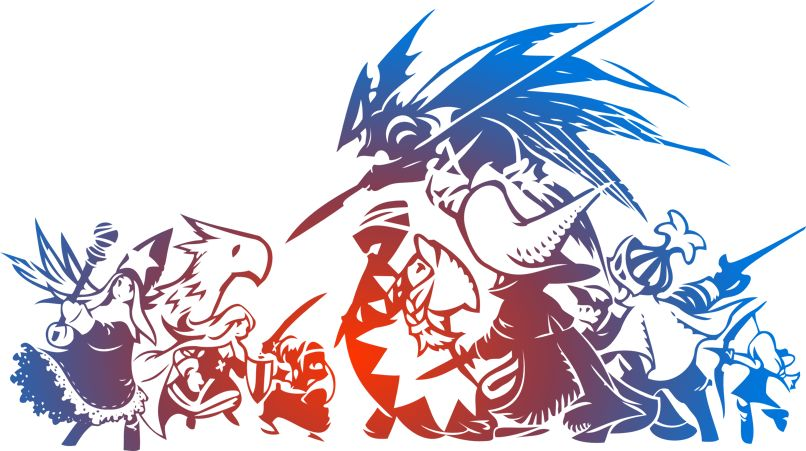
\includegraphics[width=\columnwidth]{./art/images/tactics.jpg}
%
\\\\
%
This optional rule presents the \accf{Row Combat} system as an alternative to the default combat system.
The main advantages of Row Combat are that it does not require tracking the positions of combatants on a map and it resolves battles more quickly than the default system.
However, the game is designed around the default combat system and you might run into some issues with this optional rule.
Row Combat is implemented as a set of changes on the default combat rules as listed below.
All aspects not mentioned remain unchanged.
%
\ofpar
%
The Row Combat system divides the battlefield into rows and each party has a Front Row and a Back Row.
Combatants may position themselves in either the Front Row or the Back Row before the battle commences, but the GM may enforce a layout under special circumstances, for example in surprise rounds.
Movement is absent in this system so every combatant only takes an action on his or her turn.
All effects, including Attacks, Spells, Techs and Items, that have a range of 2u or less are defined as \accf{Melee} effects and ones with a range of 3u or more are defined as \accf{Ranged} effects.
%
\ofpar
%
The \accf{Front Row} is where the maelstrom of battle takes place. 
Combatants in this row can target the opposing Front Row with all effects, but the opposing Back Row only with Ranged effects.
There is one exception to this: if the opposing Front Row is empty, then you can also target the opposing Back Row with Melee effects.
In contrast, the \accf{Back Row} is better suited for ranged combatants with lower defense.
Combatants in this row can target the opposing Front Row only with Ranged effects, but cannot reach the opposing Back Row. 
Targeting your allies, for example with supportive abilities or Items works similarly: you can target allies in your own row with all effects but allies in the other row only with Ranged effects.
%
\ofpar
%
When using effects that target an area, you can choose one additional target on the same row for each 1u of target distance. 
For example, if an effect has a target distance of 2u, you can target up to 3 combatants on the same row with it.
If the effect has a target distance of 3u or more, you can choose targets from both rows.
To use effects with the target shape Front, you have to be in the Front Row and you can only target enemies in their front Front Row. 
When using effects with target shape Line, you can always choose two targets regardless of which row you and they are in.
%
\ofpar
%
The Dash action is replaced with the \accf{Switch Row} action which you can use to switch between the Front and Back Row.
While in the Back Row, you can also use the \accf{Escape} action as follows: make an evasion check and if successful, you flee from the battle.
Furthermore, the Immobile status is replaced by Sleep in every instance and the Slow status has a new effect: you can only take an action on every other turn.
You could also encounter other effects that rely on movement or positioning. 
In these cases, the GM may reinterpret the effect in a way that works with the Row Combat system.
%
\vfill
%
\ofboxwithtitle{Example: Row Combat}
{
	Cecil and his friends fight the Magus Sisters with the current layout as shown below.
	It is Mindy's turn and she uses her Passado ability, which damages enemies in a 1u Front shape.
	She targets Cecil and Yang and afterwards ends her turn by selecting Sandy as next in order.
	Then it is Tella's turn and he uses the Ranged spell Fire and he targets Mindy with it, dealing enough damage to cause KO.
	Tella ends his turn by picking Cecil as next in order.
	Now it is Sandy's turn and she uses her Razzia ability which damages enemies in a Line shape and she targets Cid and Tella with it, causing KO to both of them.
	Then it is Cecil's turn and because the enemy Front Row is empty now, he can target the Back Row with Melee Attacks.
	He chooses to Attack Sandy and deals enough damage to KO her.
	Cindy, as the last standing Magus Sister, tries to Escape, but fails the evasion check.
	Finally, Yang takes his turn and uses the Melee Kick ability on Cindy and deals enough damage with it to cause her KO.
	The Magus Sisters are defeated!
}
%
\ofrow
%
\begin{figure}[h!]
	\centering
	\begin{tikzpicture}[]
	\tikzstyle{player}=[thick, fill=blue!15!white, draw, circle, align=center, minimum size = 0.125\columnwidth]					
	\tikzstyle{enemy}=[thick, fill=red!20!white, draw, circle, align=center, minimum size = 0.125\columnwidth]					
	
	\node[](txt)at (-0.375\columnwidth, 0.35\columnwidth) {\accf{Back}};
	\node[](txt)at (-0.125\columnwidth, 0.35\columnwidth) {\accf{Front}};
	\node[](txt)at (0.375\columnwidth, 0.35\columnwidth) {\accrf{Back}};
	\node[](txt)at (0.125\columnwidth, 0.35\columnwidth) {\accrf{Front}};
	
	\footnotesize
	\draw[color=accent, thick, dashed, -](-0.25\columnwidth, -0.3\columnwidth) -- (-0.25\columnwidth, 0.3\columnwidth);
	\draw[color=accent, thick, dashed, -](0, -0.3\columnwidth) -- (0, 0.3\columnwidth);
	\draw[color=accent, thick, dashed, -](0.25\columnwidth, -0.3\columnwidth) -- (0.25\columnwidth, 0.3\columnwidth);

	\node[player](cecil)at (-0.125\columnwidth, 0.225\columnwidth) {Cecil};
	\node[player](cid)at (-0.125\columnwidth, 0.075\columnwidth) {Cid};
	\node[player](tella)at (-0.375\columnwidth, -0.075\columnwidth) {Tella};
	\node[player](yang)at (-0.125\columnwidth, -0.225\columnwidth) {Yang};

	\node[enemy](sandy)at (0.375\columnwidth, 0.225\columnwidth) {Sandy};
	\node[enemy](cindy)at (0.125\columnwidth, 0.075\columnwidth) {Mindy};
	\node[enemy](mindy)at (0.375\columnwidth, -0.075\columnwidth) {Cindy};
	
	\end{tikzpicture}
\end{figure}
%
\clearpage